% Cap�tulo 2
\chapter{Fundamentação Teórica}

Neste capítulo será exposto os conceitos teóricos bases utilizados na construção do sistema. É válido ressaltar que cada um deles foram escolhidos mediante as experiências durante o curso.


\section{MVP (Minimal-Viable-Product)}

O Produto mínimo viável (em inglês, Minimum Viable Product) é a versão mais simples de um produto que pode ser disponibilizada para a validação de um pequeno conjunto de hipóteses sobre um negócio. 

Com esse conceito, bastante difundido dentro dos ambientes tecnológicos e de empreendedorismo, evita-se desperdício de tempo, esforço e dinheiro desenvolvendo algo que não vai atender às expectativas almejadas. Isso acontece, inclusive, em momentos em que a equipe conhece as regras de negócio relacionadas ao produto. O MVP ajuda nessa validação, orientação e no aprendizado, da forma mais rápida possível.

A ideia de MVP está originalmente vinculada aos conceitos popularizados pelo estilo Toyota de manufatura enxuta, no entanto teve maior alcance a partir da publicação do livro de Eric Ries (2011), obra essa que possui o mesmo nome do autor, durante o movimento Lean Startup. Seu objetivo é validação do primeiro passo do produto mínimo, bem menos elaborado do que sua versão final, o que é bem diferente quando comparamos com produtos criados da forma tradicional, que normalmente têm um período longo de criação de protótipo, de análise e de elaboração. O MVP foca no produto mínimo, mas que já é viável e usual, de modo que verificações possam ser feitas no grupo inicial de funcionalidades necessárias para o processo de validação de hipóteses e aprendizagem sobre o produto [2].

\section{Ruby e Ruby on Rails}

O Ruby on Rails é um framework para desenvolvimento de aplicações WEB. Criado por David Heinemeier Hansson, em 2003, a ferramenta é oriunda de um produto de sua empresa, o Basecamp. Desde então, ele se tornou muito influente e famoso, levando também a linguagem Ruby, anteriormente apenas conhecida no Japão e em poucos lugares dos Estados Unidos, a um patamar mundial.

Essa popularidade deve-se a vários fatores. Um dos principais é o fato de ser construído na linguagem de programação Ruby. Esta foi criada pelo programador e escritor Yukihiro “Matz” Matsumoto. O objetivo dele ao criar esta linguagem, em 1995, foi a de facilitar ao máximo o seu uso e o desenvolvimento com ela, levando ao programador a sensação de diversão. Matz usou a linguagem de programação Perl como inspiração, com várias referências a Smalltalk, Eiffel e Ada.

Quanto ao Rails, na época em que foi lançado, trouxe uma visão diferente ao desenvolvimento Web. Naquele momento, desenvolver para Web era cansativo, pois os frameworks eram complexos, de difícil configuração, e que acabavam por criar sistemas difíceis de se manter e de baixa qualidade [3].

David, também conhecido por DHH, ao desenvolver o Basecamp, pensou principalmente nos seguintes aspectos:

\begin{itemize}
   \item \textit{“Convention over configuration” ou convenção à configuração} -- procura-se um padrão a configuração do sistema;
   \item \textit{"Don’t Repeat Yourself”, ou “não se repita} -- deve-se evitar a repetição de código, pensando sempre no seu reaproveitamento;
   \item \textit{Automação de tarefas repetidas} -- preferir resolver uma tarefa crucial e interessante do que uma tarefa repetitiva e sem grande valor para o produto. De preferência essa última deve ser automatizada, assim aumentando a produtividade do desenvolvedor.
\end{itemize}

Esse conjunto de ideias e práticas, acabou por trazer uma maior facilidade ao desenvolvimento. É possível construir, em pouco tempo, produtos relativamente complexos. E isso foi provado pelo próprio DHH em um vídeo publicado em 2005, onde ele constrói um Blog totalmente do zero. Muitos outros frameworks, se inspiraram no Rails, como o Laravel (2011).

\section{Docker}

Na virtualização uma ou várias máquinas independentes executam virtualmente em hardware físico através de uma camada de intermediação. Diferente da virtualização, o Docker é um serviço open source de conteinerização que executa um ambiente tendo como base o próprio kernel do sistema operacional. Com essa tecnologia, largamente difundida pelo Docker, a possibilidade de criação de múltiplos ambientes isolados em um único host (mesma máquina) é possível.

Isso implica que é possível empacotar uma aplicação ou ambiente dentro de um container, possibilitando a portabilidade desse ambiente para qualquer outro host adaptado para executar o Docker. Isso assegura que o mesmo ambiente será utilizado em todos os ambientes (testes, produção, desenvolvimento), configurando apenas uma vez e replicando quantas vezes desejar.

Outro conceito importante são as imagens. Elas são os blocos de construção do mundo Docker, sendo consideradas como o código fonte dos contêineres, contendo tudo que é necessário para executar os containers, como o próprio código, bibliotecas, variáveis de ambiente e arquivos de configuração. Elas são descritas no dockerfile, que por sua vez armazena comandos que serão executados durante esse período de construção dos containers. 

Para construir ambientes mais complexos, onde são necessários diversos containers se comunicando, utiliza-se outra ferramenta chamada como Docker Compose.

\section{DevOps}

A palavra Devops originou-se da junção das palavras desenvolvedor e operação (developer and operation). Em sua definição, o Devops é uma metodologia de desenvolvimento de software que busca explorar a comunicação, a colaboração e a integração entre os desenvolvedores de software e profissionais de infraestrutura. Seu objetivo é possibilitar que a construção de sistemas se torne mais rápida e organizada, possibilitando a entrega de resultados de forma eficaz. 

Esse processo padroniza o ambiente de desenvolvimento, e eventos podem ser acompanhados com maior facilidade, objetivando manter o sistema, que já está em produção, sempre atualizado. Com isso, o desenvolvedor consegue uma maior tranquilidade enquanto desenvolve, mas sem se desligar do todo, pois os processos de implantação ou testes, por exemplo, são executados automaticamente. O objetivo é automatizar a maior quantidade possível de processos manuais em uma sequência de processos automatizados e autocontidos, sem que haja conflitos entre essas partes [7].

O uso de práticas DevOps agiliza o processo de desenvolvimento por privilegiar:
\begin{itemize}
    \item Indivíduos e interações mais do que processos e ferramentas;
    \item Produto ou serviço funcionando mais que ter documentação abrangente;
    \item Colaboração com o cliente mais que negociação de contratos;
    \item Responder às mudanças mais que seguir o plano pré-definido.
\end{itemize}

O modelo se torna responsivo a mudanças, ou seja, novas alterações no código, que são comuns na construção, não prejudicam os procedimentos de desenvolvimento. Por isso a utilização dessa prática é ideal para softwares que são constantemente atualizados, pois estes, não ficam presos a processos não adaptativos. A agilidade proporcionada estimula entregas mais frequentes, abre espaço para construção de mais testes, aumentando assim, a saúde da aplicação e a qualidade do produto final.

\section{Amazon Web Services}

O Amazon Web Services (AWS) é uma plataforma de serviços na nuvem, criada em 2006, que oferece soluções para armazenamento, redes e computação, em várias camadas. Atualmente existem diversos serviços da AWS para cada uma dessas necessidades citadas. Os que mais se destacam (e mais antigos) são o EC2 (Elastic Cloud Computer), que oferece servidores virtuais, e o S3 (Simple Storage Service), para armazenamento de arquivos. Todos os demais serviços da AWS funcionam muito bem juntos, uma vez que foram projetados para conseguirem se integrar, de modo seja possível utilizar e administrar os mais variados recursos de infraestrutura da sua aplicação, de forma descomplicada e individualmente.

Uma característica importante dos serviços da AWS é que você paga somente pelo recurso usado; não há um valor mensal fixo, ou seja, conforme a demanda, em inglês pay-per-use. E o controle pode ser feito através de uma interface web, ou também por APIs (nas mais diversas linguagens, como Python, Ruby e PHP) e linha de comando [6].

A Amazon foi a pioneira na área da computação em nuvem, chegando com uma solução que muitas empresas necessitavam: construir sistemas escaláveis com a ausência de data centers físicos dentro das empresas. Essas questões podem ser terceirizadas para a Amazon. E com a arquitetura estabelecidas por eles, a estabilidade acaba sendo certa. 1) Eles possuem data centers espalhados por todo o mundo; 2) O acesso será bem mais rápido, pois os servidores serão acionados conforme a localização dos usuários, usando a zona mais próxima dele e que possui o sistema instalado, diminuindo, assim, o tempo de resposta; 3) aplicações podem ser executadas em servidores diferentes dentro de uma região, e quando, que está sendo usado por você, parar de funcionar, outro é levantado e faz a entrega das requisições para o usuário.

\section{Scrum}

O Scrum é uma metodologia ágil para gestão e planejamento de projetos de software. Ela foi criada nos anos 90, mas só se popularizou mundialmente na década seguinte. Com isso, se tornou superior, em números de uso em empresas, do que métodos tradicionais, como o XP [8]. E essas organizações são as mais variadas, desde startups à multinacionais. Isso ocorre porque ela possui uma metodologia maleável, que não se aplica unicamente a software, embora tenha sido concebido com essa finalidade.

No Scrum, os projetos são divididos em ciclos, chamados de Sprints, que possuem um tempo definido para serem finalizadas, e que variam de acordo com a equipe e tamanho do projeto. As funcionalidades a serem implementadas são mantidas em uma lista que é conhecida como Backlog. No início de cada Sprint é realizado uma reunião de planejamento na qual o Product Owner prioriza itens dessa lista e a equipe atribui às atividades. Com uma certa frequência, é necessário que seja realizado uma breve reunião, para que assim todos possam ter conhecimento do que está sendo feito e, consequentemente, identificar impedimentos e priorizar atividades. Ao final de um Sprint, a equipe apresenta as funcionalidades implementadas, analisa o que foi feito e prepara-se o próximo ciclo. A imagem abaixo exemplifica o processo [9]:

\newpage

\begin{figure}[htb]
	\centering
  	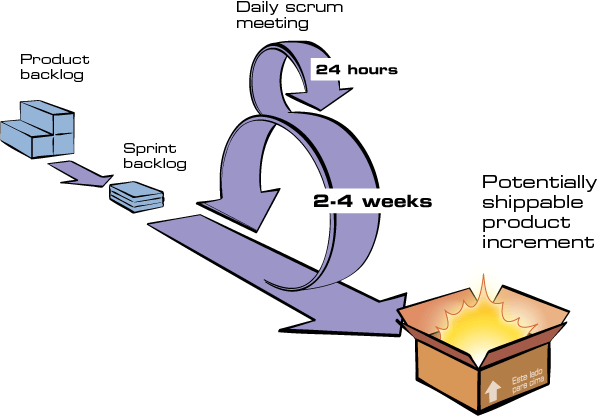
\includegraphics[scale=0.60]{src/imagens/scrum.png}
  	\textsf{\caption{Esquema do funcionamento do Scrum}}
  	\label{fig:FiguraTeste}
\end{figure}


Os benefícios no uso do Scrum incluem:
\begin{itemize}
    \item Entregas frequentes aos clientes;
    \item Construção do projeto mais segura;
    \item Qualidade do produto aumentada;
    \item Controle do progresso do projeto;
    \item Redução do desperdício;
    \item Aumento de produtividade.
\end{itemize}

\section{Teste Unitários}

Test-Driven Development (TDD) é uma das práticas de desenvolvimento de software sugeridas por diversas metodologias ágeis, como XP. A ideia por trás dele é bem simples: escrever testes antes mesmo de escrever o código de produção. Dessa forma, o desenvolvedor garante que boa parte do seu sistema tem um teste que aumenta a garantia do seu funcionamento [14]. A prática de TDD agrega muitos benefícios ao processo de desenvolvimento.

Muitos são os benefícios da utilização do TDD. Uma das principais diz respeito a qualidade externa do produto. A bateria de testes automatizados gerados pela prática dá mais segurança ao desenvolvedor na hora de mudanças, pois garante que possíveis erros gerados ao se construir uma grande funcionalidade, ou modificar alguma coisa, sejam logo identificados. Além disso, escrever testes de unidade forçará o desenvolvedor a escrever um código de maior qualidade pois, para escrever bons testes unitários, o desenvolvedor é obrigado a fazer bom uso de orientação a objetos. A prática ajuda a escrever um bom software, com um nível qualidade superior, mais fácil de ser mantido e evoluído.

A mecânica na prática se baseia no ciclo Vermelho-Verde-Refatorar. Quando se inicia uma tarefa, é preciso inicialmente criar um teste unitário, que nada mais é do que um trecho de código que deixa claro o que determinado trecho de código deve fazer. Como não foi implantado da funcionalidade em si, o teste irá falhar. O desenvolvedor então trabalha com o mínimo necessário para fazer esse teste passar. A próximo fazer é a refatoração desse código é melhorar o código que já está escrito. A cabeça do desenvolvedor é complicada: quando ele está focado em implementar a funcionalidade, ele raramente está pensando também em qualidade de código. Não tem jeito, é assim que funcionamos. E justamente por isso que, após a implementação da funcionalidade, o desenvolvedor para e melhora a qualidade do código (que já funciona e atende ao requisito do negócio) [14].
